\def\theTopic{ESP}
\def\dayNum{5}
\begin{center}
{\bf {\large Can Humans Sense Each Others' Thoughts?}}\\
\vspace{-.1in}
\end{center}


Mind readers often appear in spooky SciFi movies. (Insert spooky music
here.)  Is it
possible that some people can read minds? In the 1930's
Dr.~J.B.~Rhine at Duke University designed experiments to see if some
undergraduate students could tell which card (see the five ``Zener''
cards below) a ``sender'' was looking at. The deck of cards (5 of each
type) was shuffled and a card drawn at random. After each attempt, the
card was returned to the deck and the deck was reshuffled (we call
this sampling with replacement).  Therefore each of the five card types has
an equal chance of occurring at any draw. 
\begin{center}
  
\includegraphics[width=.5\linewidth]{plots/Zener_cards.png}
\end{center}

 Rhine found one exceptional subject in his extrasensory perception
 (ESP) research, Adam Linzmayer, an economics undergraduate at Duke.
 Linzmayer went through the experiments in 1931, and correctly
 identified 36\% of 25 cards as the ``receiver'' in the study.   We will
 start by investigating this student's result as Rhine did, hoping to
 prove that Linzmayer does have extrasensory perception. 

{\bf Step 1. State the research question. }\\
1. Based on the description of the study, state the research question.
\begin{students}
  \vspace{2cm}
\end{students}

\begin{key}
{\it  Can any person tell what someone else is looking at with no
  other form of communication?.}
\end{key}



{\bf Step 2. Design a study and collect data.}\\
 Linzmayer correctly identified the card 9 out of 25 times in one
 trial.\vspace{-.3cm}
 \begin{enumerate}
   \setcounter{enumi}{1}
   \item  What were the possible outcomes for 1 attempt (guessing one card)
     that Rhine would have recorded?
\begin{students}
  \vspace{1cm}
\end{students}

\begin{key}
{\it Right or Wrong}
\end{key}

\item Your answer above gives the outcomes of the variable of interest
  in the study.  Is this variable quantitative or categorical?
\begin{students}
  \vspace{1cm}
\end{students}

\begin{key}
{\it Categorical}
\end{key}
  
   \end{enumerate}
   
{\bf Step 3. Explore the data. }\\
With categorical data, we  report the number of “successes”
or the proportion of successes as the ``statistic'' gathered from the
sample.  
 \begin{enumerate}
   \setcounter{enumi}{3}
   \item   What is the sample size in this study?  $n = $ 
\begin{students}
  \vspace{1cm}
\end{students}

\begin{key}
{\it 25 guesses}
\end{key}

   \item  Determine the observed statistic and use correct notation to
     denote it. 
\begin{students}
  \vspace{1cm}
\end{students}

\begin{key}
 $\phat = 0.36$
\end{key}

   \item  Could Linzmayer have gotten 9 out of 25 correct even if he
     really didn't have ESP and so was randomly guessing between the
     five card types? 
\begin{students}
  \vspace{1cm}
\end{students}

\begin{key}
{\it Yes, it is possible to do that well just by chance.}
\end{key}

   \item  Do you think it is likely Linzmayer would have gotten 9 out of 25
     correct if he was just guessing randomly each time?  
\begin{students}
  \vspace{1cm}
\end{students}

\begin{key}
{\it No.}
\end{key}

   \end{enumerate}
   
{\bf Step 4. Draw inferences beyond the data. }\\
Two things could have happened:\vspace{-.5cm}
\begin{itemize}
\item He got over one third correct just by  random chance -- no
  special knowledge.  
\item He is doing something other than merely guessing and perhaps has ESP.
\end{itemize}

 \begin{enumerate}
   \setcounter{enumi}{7}
   \item   Of the two possibilities listed above, which was Rhine
     trying to demonstrate (the alternative) and which corresponds to
     ``nothing happening'' (the null)? 
\begin{students}
  \vspace{1cm}
\end{students}

\begin{key}
{\it Rhine hoped to show Linzmayer actually had ESP (alternative),
  rather than that he was just guessing (the null).}
\end{key}

\item\label{trueESP-p} What is the value of the true parameter if
  Linzmayer is picking a card at random? Give a specific value and use
  correct notation to denote it. 
\begin{students}
  \vspace{1cm}
\end{students}

\begin{key}
$p = 1/5 = 0.20$
\end{key}


   \item If Linzmayer is not just guessing and did have ESP, what
     values might the true proportion take on?  Again, use correct notation to
     denote this range of values. 
\begin{students}
  \vspace{1cm}
\end{students}

\begin{key}
$(0.20, 1.00)$
\end{key}
     Is the observed statistic (9/25) in this interval?
\begin{students}
  \vspace{0.4cm}
\end{students}

\begin{key}
{\it Yes}
\end{key}


   \item \label{ESP-hyps} When writing the null and alternative
     hypotheses, we may use words or we may use symbols.  Rewrite the
     null and alternative hypotheses in both words and notation by
     combining your answers
     from 8 -- 10.\\
     $H_0$:
\begin{students}
  \vspace{1.2cm}
\end{students}
\begin{key}
{\it $p = 0.20$}
\end{key}
\\
     $H_a$:
\begin{students}
  \vspace{1.2cm}
\end{students}
\begin{key}
{\it $p > 0.20$}
\end{key}
\\
     \item Think of a ``spinner'' on a game board. How would you
       subdivide and color it so that each spin would be equivalent to
       Linzmayer randomly guessing one card and getting it right/wrong
       with the null hypothesis probability.  (Hint: you do not need 5
       segments.) Sketch your spinner on the circle below and shade the area
       where he gets it right just by chance. Put a paper clip on the
       paper with pen to hold one end on the center.  Spin 25 times
       and count the number of successes.

       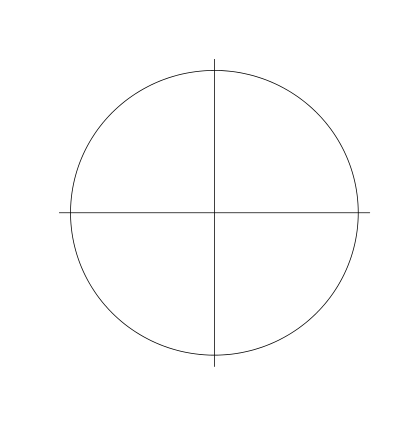
\includegraphics[width=.3\linewidth]{plots/spinnerCircle.png}
 % png("plots/spinnerCircle.png",height=400,width=400)
 % plot(cos(myValues),sin(myValues), type = "l", xlab = "", ylab = "", axes=FALSE, bty="n")
 % abline(h=0); abline(v=0)
 % dev.off()
\vspace{-1cm}

  \item Now we'll use a web app to speed up the process.  Go to
     \url{http://shiny.math.montana.edu/jimrc/IntroStatShinyApps/} and click
       ``Enter / Describe Data'' under the ``One Categ.'' menu.
       Enter the counts to show how many Linzmayer got right and got
       wrong. (These should add up to 25, but neither is 25.)
       Click ``Use These Data'' and record his proportion correct.

\begin{students}
  \vspace{1cm}
\end{students}
\begin{key}
{\it $\phat = 0.36$}
\end{key}

   \item Now from the ``One Categ.'' menu choose ``Test''. and enter
     the value from \ref{trueESP-p} as the True Proportion.   Run 5000 samples
       and sketch the plot below.

\begin{students}
  \vspace{2cm}
\end{students}

\begin{key}
  \includegraphics[width = .5\linewidth]{plots/Esp-5001Draws.png}
\end{key}

     \item Check the summary statistics inside the plotting window.
       Does the mean agree with the null or alternative hypothesis?
       Explain why it should.
\begin{students}
  \vspace{1.2cm}
\end{students}
\begin{key}
{\it My mean is 0.199, which is darn close to 0.20. They should agree
  because the simulations were created by assuing $H_0$ is true.}
\end{key}
\\

     \item What proportion did Linzmayer get correct? \\
           Type that value in to the box just after ``than'' below the
           plot.  Select the direction (less, more extreme, or more)
           based on the alternative hypothesis in
           \ref{ESP-hyps}. Click \fbox{Go} and record the proportion of
           times this occurred.\\  
           Would you consider this an unlikely result?
\begin{students}
  \vspace{1.2cm}
\end{students}
\begin{key}
{\it $\phat = 0.36$, I got 226 results of 5001 that
  were this extreme (p-value = 0.045), so doing this well is pretty unlikely.}
\end{key}
\\

     \item  Go back to figure \ref{fig:SOE-pvalue} to report the
       strength of evidence against $H_0$.  Give the numeric and the
       verbal strength of evidence.  
\begin{students}
  \vspace{1.2cm}
\end{students}
\begin{key}
{\it The p-value we observed is 0.045, which gives ``moderately
  strong'' evidence against $H_0$. }
\end{key}
\\
\end{enumerate}



% {\bf 3S Strategy for Measuring Strength of Evidence}\vspace{-.4cm}
% \begin{enumerate}
% \item  Statistic: Compute the statistic from the observed sample data. 
% \item  Simulate: Identify a ``by chance alone'' explanation for the
%   data. Repeatedly simulate values of the statistic that could have
%   happened when the chance model is true. 
% \item  Strength of evidence: Consider whether the value of the
%   observed statistic from the research study is unlikely to occur if
%   the chance model is true. If we decide the observed statistic is
%   unlikely to occur by chance alone, then we can conclude that the
%   observed data provide strong evidence against the plausibility of
%   the chance model. If not, then we consider the chance model to be a
%   plausible (believable) explanation for the observed data; in other
%   words what we observed could plausibly have happened just by random
%   chance. 
% \end{enumerate}


% Let’s review how we have already applied the 3S strategy to this study.
% \begin{enumerate}
% \setcounter{enumi}{17}
% \item Statistic. What is the statistic in this study?\vspace{.62cm} 
% \item  Simulate. Describe the three inputs we had to give the web app
%   and the results it returned. \vspace{2cm} 
% \item  Strength of evidence. What feature of the app's output gave the
%   p--value? \vspace{2cm} 

% \end{enumerate}

{\bf Step 5: Formulate conclusions.}\\
 Based on this analysis, do you believe  that Linzmayer was just
 guessing? Why or why not? 

\begin{students}
  \vspace{2cm}
\end{students}
\begin{key}
{\it This is fairly strong evidence that he was not just guessing.}
\end{key}

Are there ways other than ESP that a person could do well as a ``receiver''?
Explain. 

\begin{students}
  \vspace{1.2cm}
\end{students}
\begin{key}
{\it Yes, he could be cheating in some way.}
\end{key}


Another part of the scientific method is a reliance on replication.
Other scientists tried to replicate this study and could not find
another person like Linzmayer. 



{\bf Take Home Messages}
\begin{itemize}
\item 
This activity was much like the previous one (Helper--Hinderer),
except that the null hypothesis value was not one-half. (Here ``at
random'' was 1 of 5, not 1 of 2)
\item 
Again note how $H_0$ is used to compute the p--value.  The alternative
comes into play only when we need to see which direction to count as
``more extreme''.
\item 
Both examples we've done so far have used a $>$ alternative, but that
is not always the case.
\item 
And finally: other reporting on Linzmayer suggests that he was
cheating, rather than reading minds.
 \item 
  Use the remaining space for any questions or your own summary of the
  lesson. 

\end{itemize}




